\section{State vector simulator}
\label{statevector_section}
We first implement the algorithm locally on a simulator. Firstly, we use \emph{State vector simulator}.
The StateVectorSimulator as part of the IBM Qiskit and it does not really simulate a quantum system.
It essentially does all the algebraic operations and does only one run of the circuit to give us the final state.
So there is no quantum randomness here.
Thus, it becomes a handy tool in following the evolution of the exact state of the system.%

\begin{minipage}{0.5\textwidth}
    \begin{figure}[H]
    \centering
    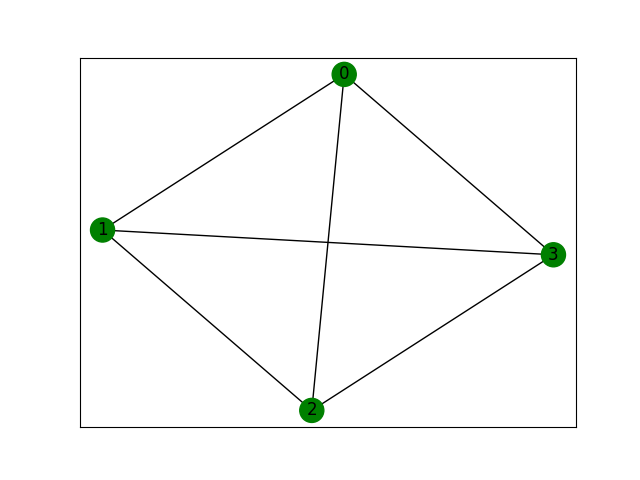
\includegraphics[width=0.5\textwidth]{images/4ngraph.png}
    \caption{4-n regular graph}
    \label{fig:4ngraph}
    \end{figure}
\end{minipage}
\begin{minipage}{0.45\textwidth}
Consider the following 4-n regular graph as shown in figure \ref{fig:4ngraph} for our analysis here.
Here, it is evident that the partitions with Maximum cost correspond to the following states : $\ket{0011}, \ket{0101}, \ket{0110}$ and the states with essentially the same partition but exchanging all the nodes, i.e, $\ket{1100}, \ket{1010}, \ket{1001}$. All of them have a cut of size 4.
\end{minipage}

In figure \ref{fig:UC1} it is evident that the probabilities do not change upon application of $U_C$ as discussed earlier.
It is only after the application of the \emph{mixing operator}, showed in \ref{fig:UB1}, that the probabilities change.
And we can also see that the states which correspond to higher cost have higher probabilities here in figure \ref{fig:UB1}.

\begin{figure}[H]
    \begin{minipage}{0.5\textwidth}
        \centering
        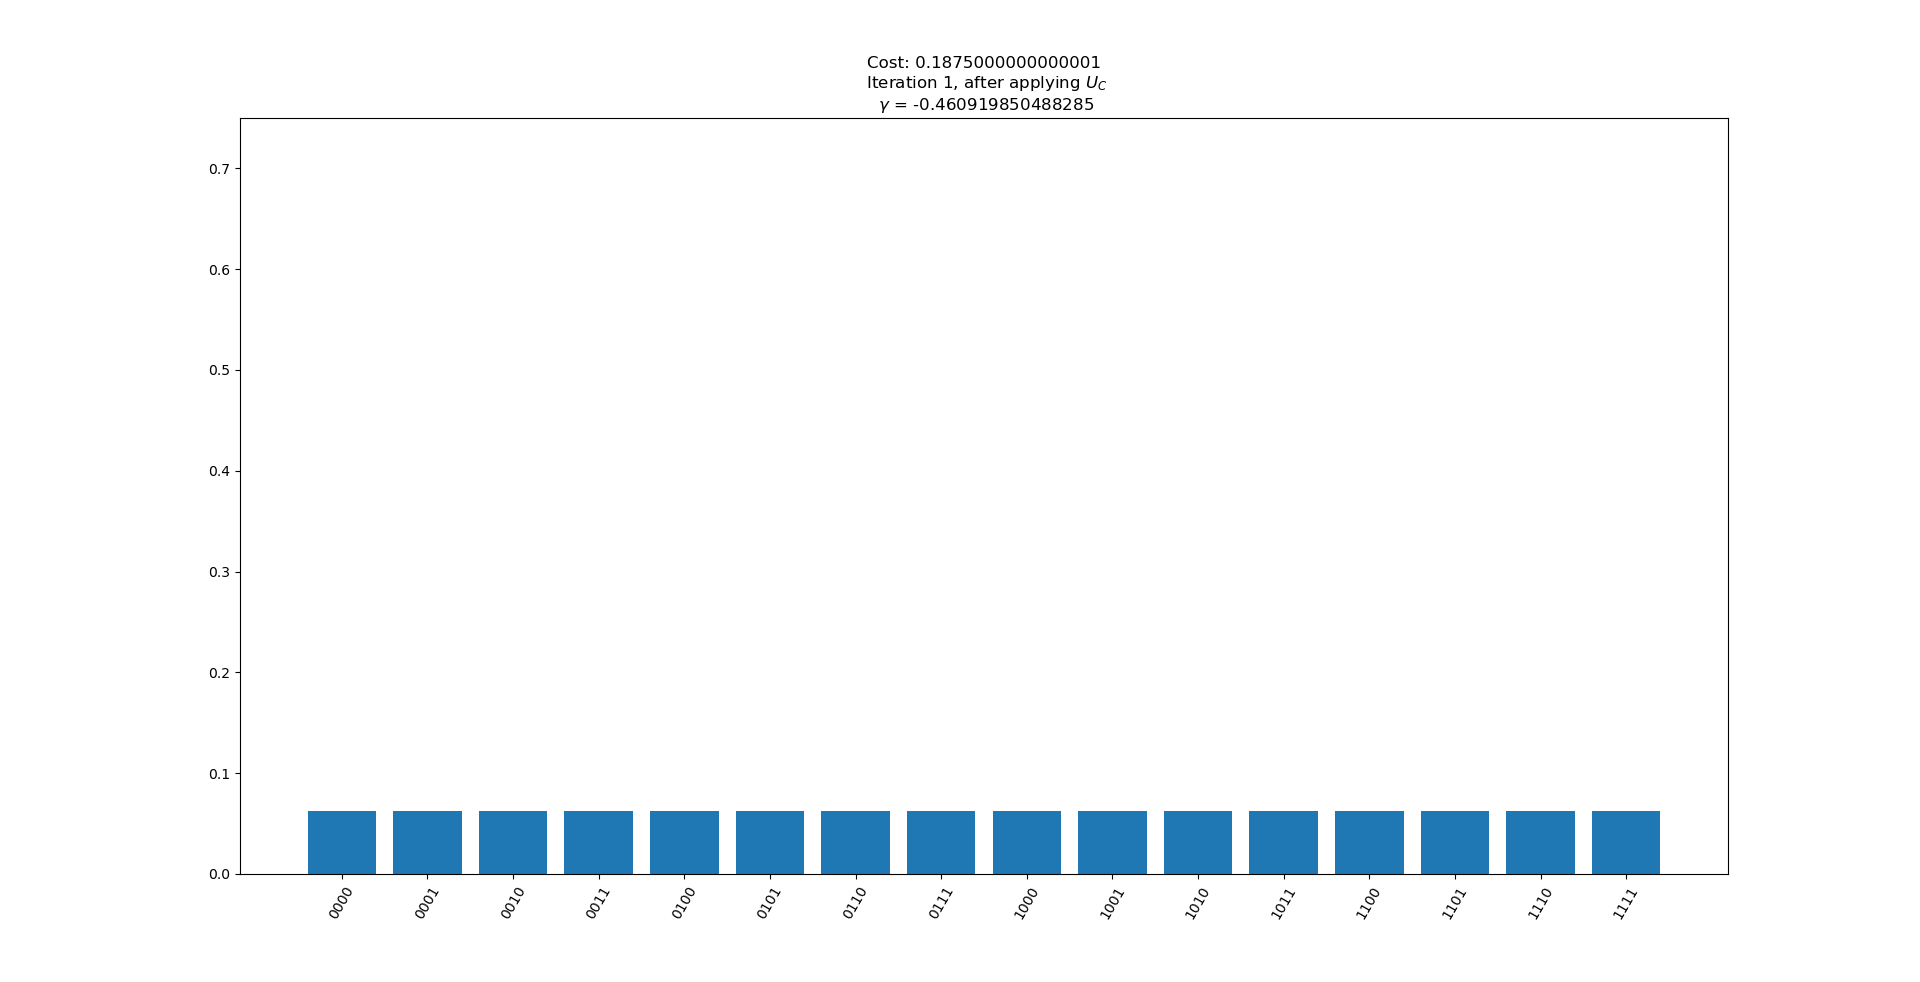
\includegraphics[width=\textwidth, height= 4.8cm]{1.png}
        \caption{Resulting state after $U_C$: $U_C\ket{+}^{\otimes 4}$\\
                $\gamma = 3.633$, $\langle C \rangle =3$}
        \label{fig:UC1}
    \end{minipage}
    \begin{minipage}{0.5\textwidth}
        \centering
        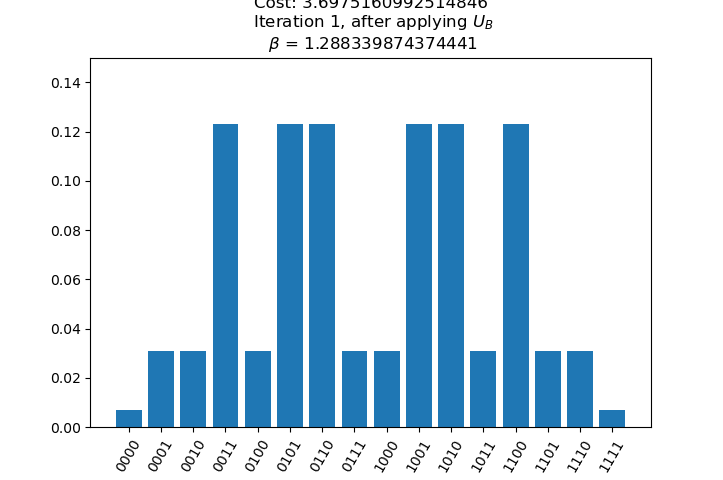
\includegraphics[width=\textwidth, height= 4.8cm]{2.png}
        \caption{Resulting state after $U_B$: $U_BU_C\ket{+}^{\otimes 4}$\\
                $\beta = 4.995$, $\langle C \rangle =3.798$}
        \label{fig:UB1}
    \end{minipage}
\end{figure}

We can see similar analysis for more than one layers. It can be seen that for an ideal case (without noise), as with the state vector simulator, the performance should monotonically increase with increasing p.
Say the approximation ratio after $p$ layers is $\alpha_p$, then,
$$\alpha_{p+1} \geq \alpha_p$$
since we can have for the $(p+1)^{th}$ layer, $(\beta_{p+1}, \gamma_{p+1}) = (0, 0)$.
And in that case, it is same as essentially applying only $p$ layers.
Note, that this is only true if there is no noise and we explore the performance in presence of noise further in the sections that follow.

For the same 4-n regular graph shown in figure \ref{fig:4ngraph}, we see the evolution of state vector for $p = 2$ layers.

\begin{figure}[H]
    \centering
    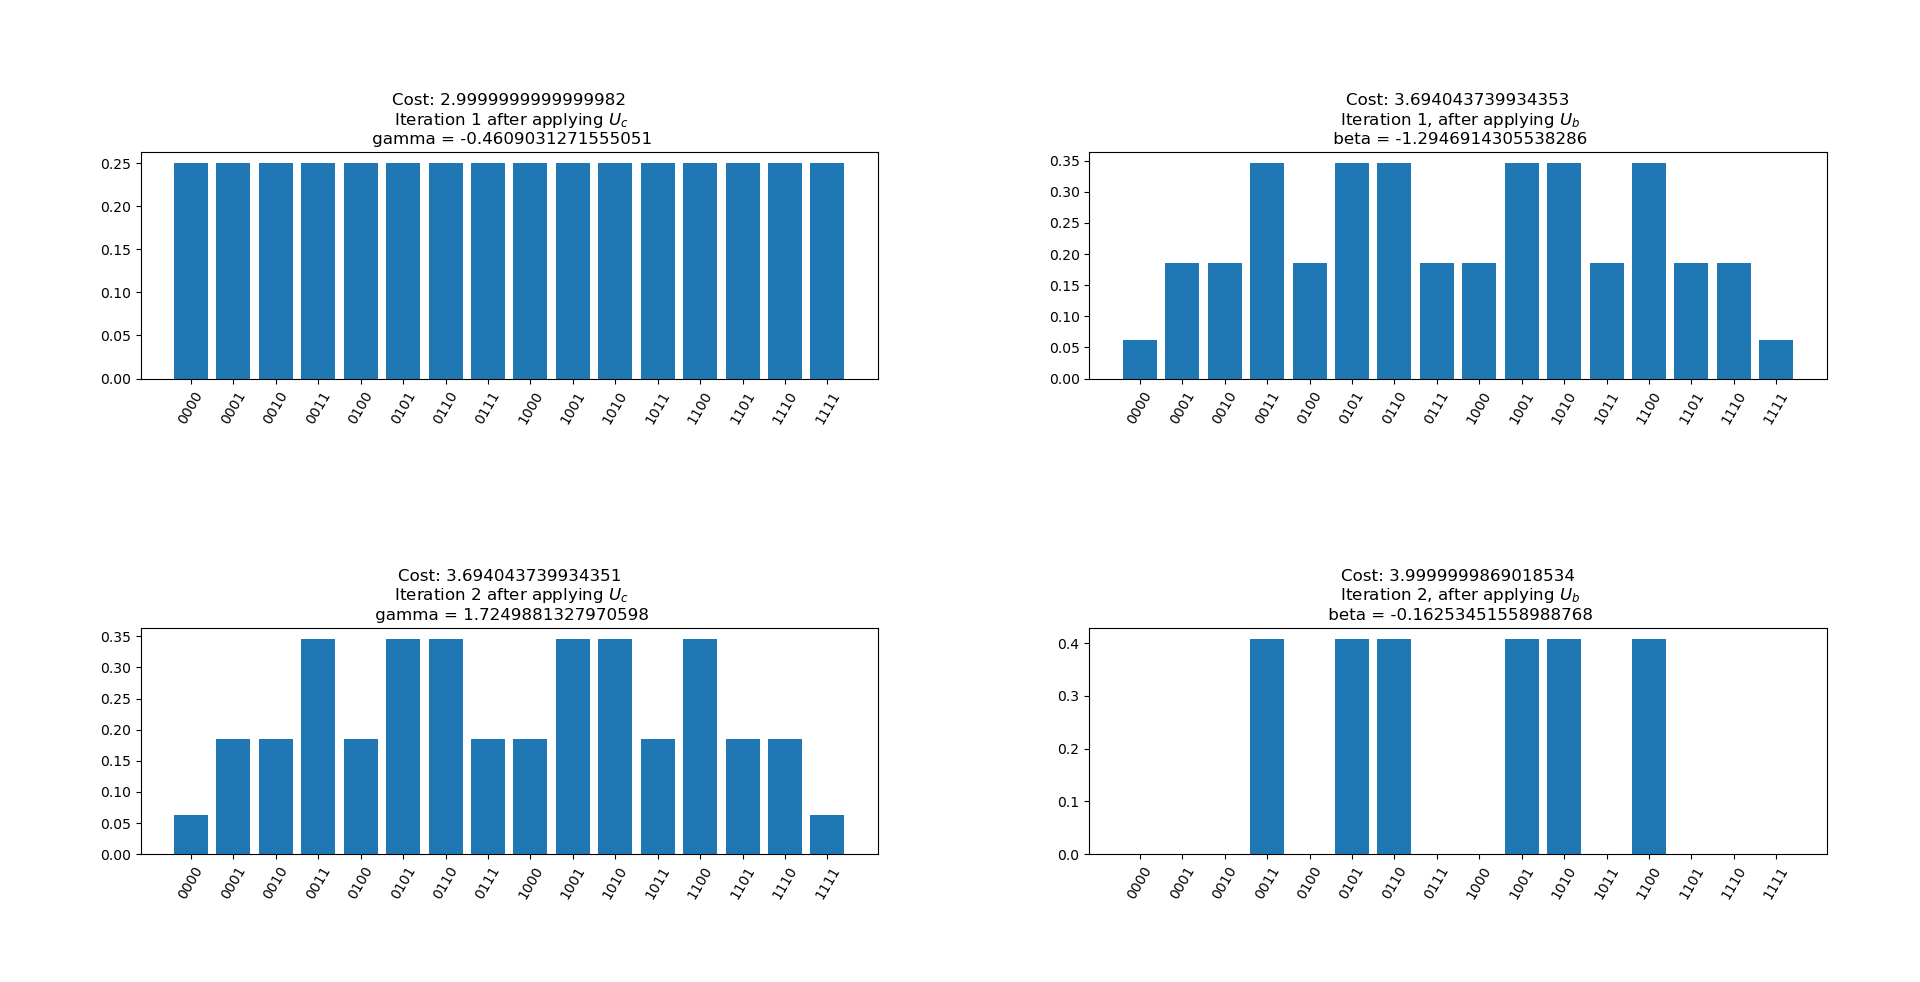
\includegraphics[width= \textwidth,  height= 7.9cm]{Figure_2.png}
    \caption{One possible evolution of state vector to the optimum solution for 4n regular graph for $p = 2$ layers\\
    $\vec{\gamma} = [3.633, 4.867]$, $\vec{\beta} = [4.995, 6.121]$ and $\langle C \rangle = 4$}
    \label{fig:stvc_lbl}
\end{figure}

We note that for $p = 2$, after applying the gates in both the \textit{layers}, with probability almost equal to 1, we get the states with the maximum cost. Thus, we always find the MaxCut in this case.
One interesting feature we see in figure \ref{fig:stvc_lbl}, is the that the optimizer keeps the same $\gamma_1$ and $\beta_1$ for both the cases i.e, when we had $p = 1$ and now that we have $p = 2$.
But this need not be the case. There could be other \textit{optimization paths} that the optimizer can take.
This can be seen in the following figure \ref{fig:my_label}
 
 \begin{figure}[H]
     \centering
     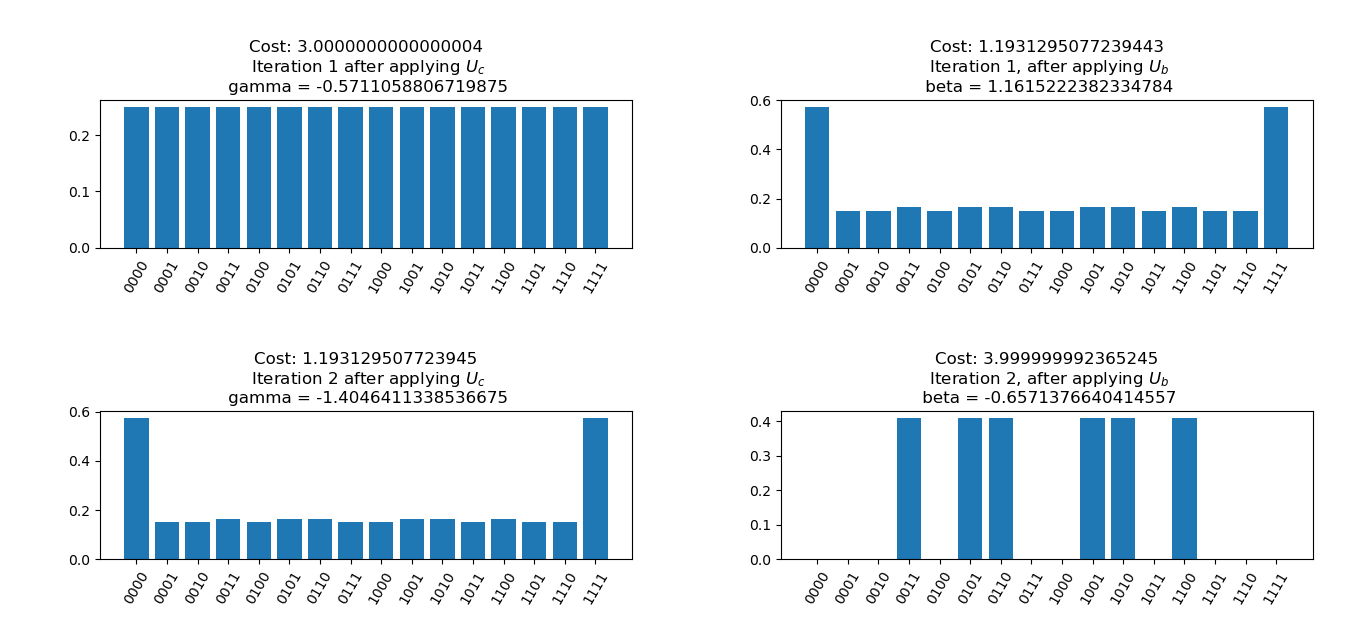
\includegraphics[width= \textwidth, height= 7.9cm]{Figure_1.png}
     \caption{Another evolution of state vector to the optimum solution for 4n regular graph for $p = 2$ layers\\
    $\vec{\gamma} = [5.718, 1.329]$, $\vec{\beta} = [5.545, 0.56]$ and $\langle C \rangle = 4$}
     \label{fig:my_label}
 \end{figure}
 
Thus, with different optimization paths taken, we can reach the same optimum solution.
 
 \begin{figure}[h]
    \begin{minipage}{0.33\textwidth}
        \centering
        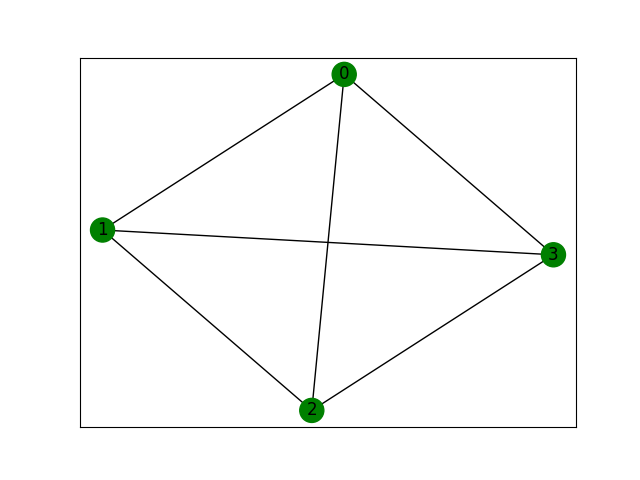
\includegraphics[width=\textwidth]{images/4ngraph.png}
        \caption{4-nodes regular graph}
        \label{fig:4n}
    \end{minipage}
    \begin{minipage}{0.33\textwidth}
        \centering
        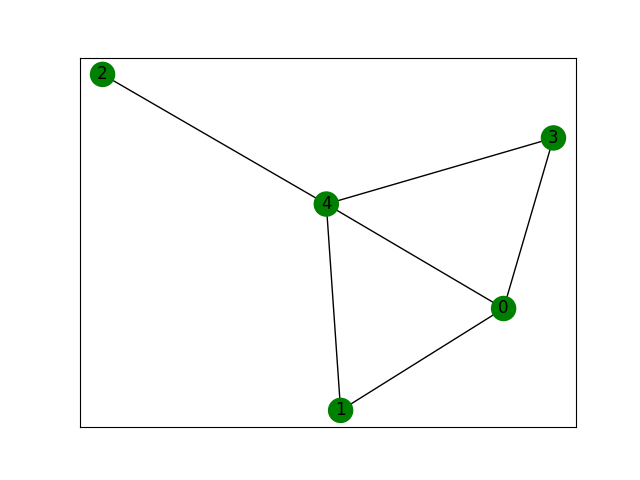
\includegraphics[width=\textwidth]{images/erdos renyi n = 5.png}
        \caption{5-nodes Erdos Renyi}
        \label{fig:er5}
    \end{minipage}
    \begin{minipage}{0.33\textwidth}
        \centering
        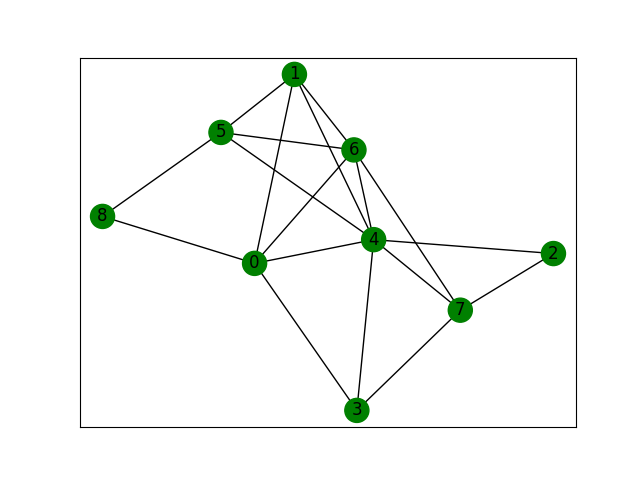
\includegraphics[width=\textwidth]{images/Erdos-Renyi graph.png}
        \caption{9-nodes Erdos Renyi}
        \label{fig:er9}
    \end{minipage}
\end{figure}

For the ideal case, we also look at other more complex graphs and see the performance of QAOA.
At the top of the page, in the figure \ref{fig:4n}, we have the 4n regular graph that we considered up until now. Additionally, in figure \ref{fig:er5} and \ref{fig:er9}, we see a 5-node and 9-node graph generated using the Erdos Renyi random graph model.
 \begin{wrapfigure}{l}{0.66\textwidth}
    \centering
    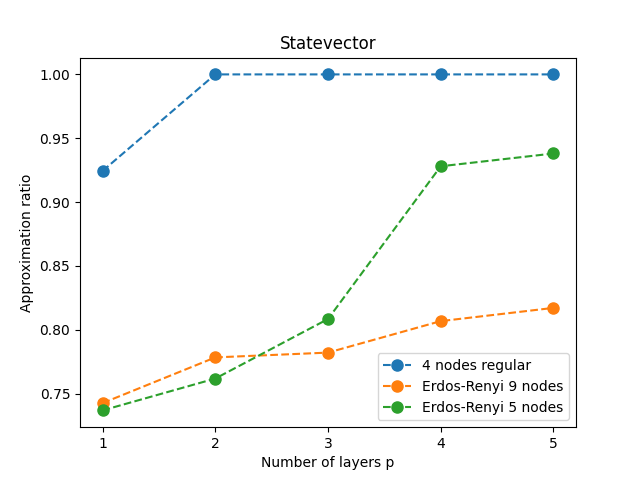
\includegraphics[width=0.66\textwidth]{images/StateVector.png}
    \caption{Comparison between the results for different graphs.}
    \label{fig:statevector_graph}
\end{wrapfigure}

As the figure on the left shows, the performance of the algorithm (measured as the ratio between the expectation value obtained and the actual max cut of that graph) is not as high for small values of p for more complex graphs.
We can also note that, as expected, the performance increases with the number of layers $p$.\\
Thus, for more complex problems, one would require sufficient number of layers to actually solve the MaxCut or any similar combinatorial optimization problem.
But, increasing $p$ is not only computationally expensive, but there are also errors which play a bigger role as circuit depth and complexity increases.

To finally include the noise that we have talked about until now, we can not use the StateVectorSimulator.
We use an actual quantum simulator next and analyse the result.

\section{QASM simulator}
\label{qasm_section}
We use QASM simulator provided by Qiskit and implement the algorithm.
We again consider the same 4n regular graph as earlier.
We use a simple noise model at first. We consider only depolarising error and see how the extent of depolarisation affects the performance. The depolarising error can be characterised as:

\[
    \rho \Rightarrow (1-\lambda)\rho + \lambda \frac{\mathds{1}}{d}\text{,}\quad \text{with } \rho = \ket{x}\bra{x}
\]
Here $\lambda \in [0, 1]$ is the \emph{depolarizing factor}. Greater the value of $\lambda$, greater is the depolarisation.

 \begin{wrapfigure}{r}{0.66\textwidth}
    \centering
    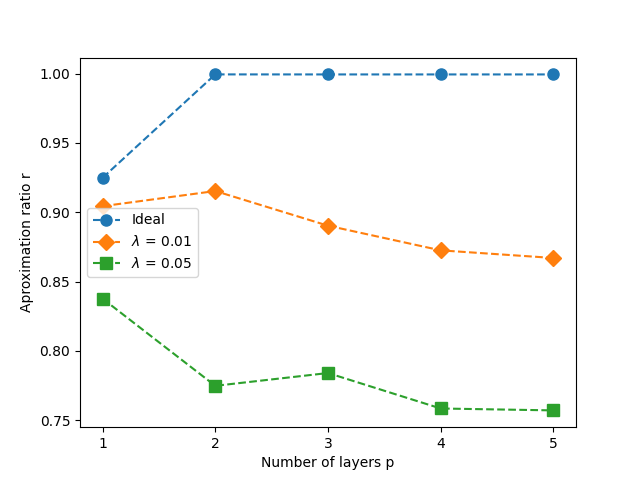
\includegraphics[width=0.66\textwidth]{images/depolarizing noise.png}
    \caption{Depolarizing noise running the algorithm for the regular 4-nodes graph.}
    \label{fig:dep_err_per}
\end{wrapfigure}
The figure \ref{fig:dep_err_per} on the right compares the performance for different values of $\lambda$.

Firstly we can see how QASM gives the same results for the ideal case that we observed in StateVector simulator earlier, as is expected.
But what this simulation reveals for noisy system is that the performance does not necessarily go up with increasing $p$.
We also see that for more noise, the algorithm is performing worse, as is expected.
Not only do the errors add up as the number of operations increase with the circuit depth increases, but as the circuit depth increases, the execution time also goes up and then we see more depolarisation.
We also see that for smaller values of $\lambda$, we get optimum performance for $p=2$ but for greater noise ($\lambda = 0.05$ here), we in fact get optimum performance for $p = 1$.
Tying this to our analysis in previous section for more complex systems \ref{fig:statevector_graph}, this implies that even though we need more number of layers for better performance, using more layers will be counterproductive since the increasing error due to noise disincentivizes using more layers, as we see here.

Thus far, we have only considered only depolarising error, we further consider more complex errors and try to \textit{mimic} a real quantum hardware.

\section{Fake Vigo}
\label{fakevigo_section}

The optimisation process in QAOA requires a high number of calls to the objective function. Therefore, before we run it on an actual hardware backend, it is practical to first run it on a simulator with a noise model as close to the actual noises as possible to be able to gauge the performance and to get an idea about what to expect. In this section we use a built in noise model provided with Qiskit called \texttt{FakeVigo}. This is a noise model based on the IBM's Quantum device \texttt{Vigo} and thus the name \texttt{FakeVigo}.


FakeVigo noise model includes the following errors:
\begin{itemize}
    \item \textbf{Single-qubit gate errors} consisting of a single qubit depolarizing error followed by a single qubit thermal relaxation error.
    \item \textbf{Two-qubit gate errors} consisting of a two-qubit depolarizing error followed by single-qubit thermal relaxation errors on both qubits in the gate.
    \item \textbf{Single-qubit readout errors} on the classical bit value obtained from measurements on individual qubits.
\end{itemize}

\newpage

 \begin{wrapfigure}{l}{0.66\textwidth}
    \centering
    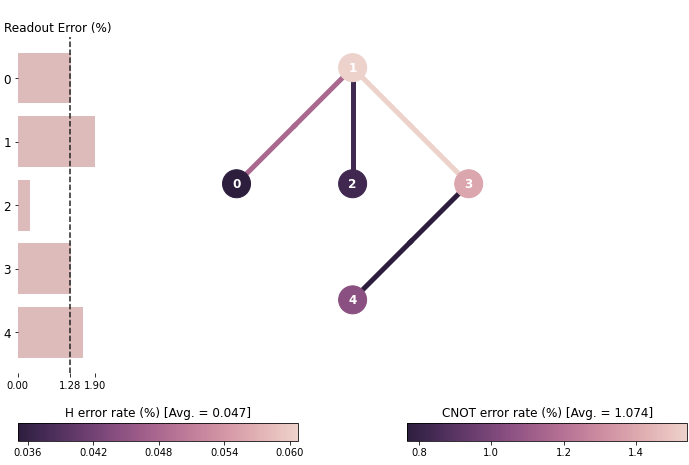
\includegraphics[width=0.5\textwidth]{images/fakeVirginMap.png}
    \caption{Fake Vigo error map provided by Qiskit.}
    \label{fig:error}
\end{wrapfigure}

Thermal relaxation takes in account the T1 time (also known as energy relaxation time) and T2 time (also known as dephasing time). These two parameters account for the overall decoherence error the qubit suffers. On figure \ref{fig:error} we can see a detailed error map provided by Qiskit which shows the error parameters and how they change for each qubit. Furthermore, the thermal relaxation, which are not included in the figure, are obtained from the documentation\cite{vigo_ref}.

Thus, we do similar analysis as we did for simple depolarising error and plot the results as shown in figure \ref{fig:4n_fakeV}.

Here we see that for a realistic noise model, the performance does not actually increase with increasing $p$ but it instead falls.
This points out the fact that our system is too erroneous and that the increase in performance due to more layers is not sufficient to overcome the decrease in performance due to errors.

\begin{figure}[h]
    \centering
    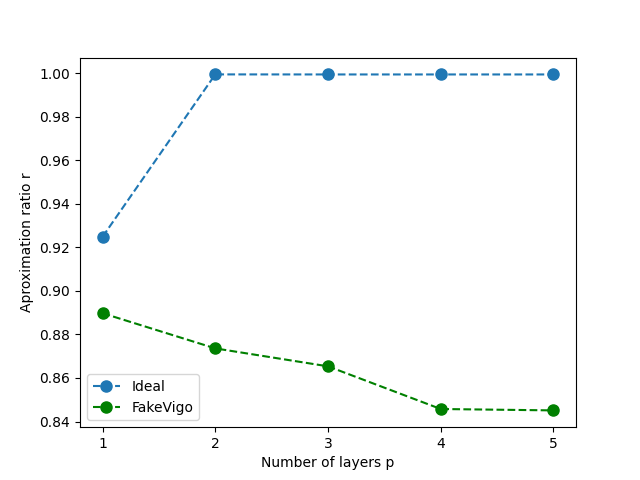
\includegraphics[width=0.5\linewidth]{images/4 node regular graph with fake vigo.png}
    \caption{Comparison of approximation ratio for \texttt{FakeVigo} and ideal case (no noise) for 4n regular graph for up to $p = 5$.}
    \label{fig:4n_fakeV}
\end{figure}

%%%%%%%%%%%%%%%%%%%%%%%%%%%%%%%%%%%%%%%%%%%%%%%%%%%%%%%%%%%%%%%%%%%%%%%%%%%%%%%%%%%%%%%%%%%%%%%%%%%%%
\section{Hardware Backend}
\label{hardware_section}

Up until now we have been running the algorithm on classical simulators. As a next step we will run it on real hardware. As mentioned earlier, we have chosen the IBM Quantum Experience's machine \textit{Vigo} \cite{vigo_ref}, a 5-qubit quantum processor (see figure \ref{vigo}). 

The first thing we need to realize is that in a real quantum computer not all the qubits are connected. This means that it is not possible to apply 2-qubit gates directly between any two arbitrary qubits. To apply 2-qubit gates between qubits that are not connected some intermediate gates (SWAP gates) are needed. This considerably increases the circuit depth and, as a consequence, the overall error. We will again apply our algorithm to the 4-n 3 regular graph, so it is easy to see that the shapes of the graph (figure \ref{fig:4ngraph}) and Vigo (figure \ref{vigo}) do not match, meaning that the compiler will indeed add intermediate SWAP gates that will increase the overload of the circuit.


In addition, we face another issue when running the algorithm on real backends: the time needed to run a job in IBM Quantum Experience. As most of the current backends nowadays, IBM's machines are only accessible via cloud. Therefore, when you submit a job to an IBM's machine it enters a queue with jobs from other users before eventual execution. The order in which these jobs are executed is decided through a fair-share queuing formula, which means that the more complex your job is the more time it will take to be executed. As QAOA is an optimization algorithm, it takes many evaluations to the objective function to reach the optimal value of all the $\gamma$ and $\beta$. Each of these evaluations of the objective function will be queued with a waiting time around 1-4 minutes, so the time needed to run the entire algorithm escalates very quickly with the number of layers.

Therefore, it is key to come up with ideas to reduce the number of function evaluations the optimizer takes. Many approaches have been taken in this direction, as for example in \cite{alam2020accelerating} where a machine  learning based approach is taken to accelerate the QAOA convergence through feature extraction. In this project we have addressed this problem with two different ideas: \textit{layer by layer optimization} and a \textit{smart choice of the optimizer}. 


 \begin{figure}
 
    \begin{minipage}{0.5\textwidth}
    \centering
    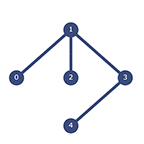
\includegraphics[width=.5\textwidth]{Vigo.png}  
  \captionsetup{width=.8\linewidth}
    \caption{Schematic representation of the connectivity of the qubits in Vigo. Retrieved from \cite{vigo_ref}}
    \label{vigo}
    \end{minipage}\begin{minipage}{0.5\textwidth}
    \centering
    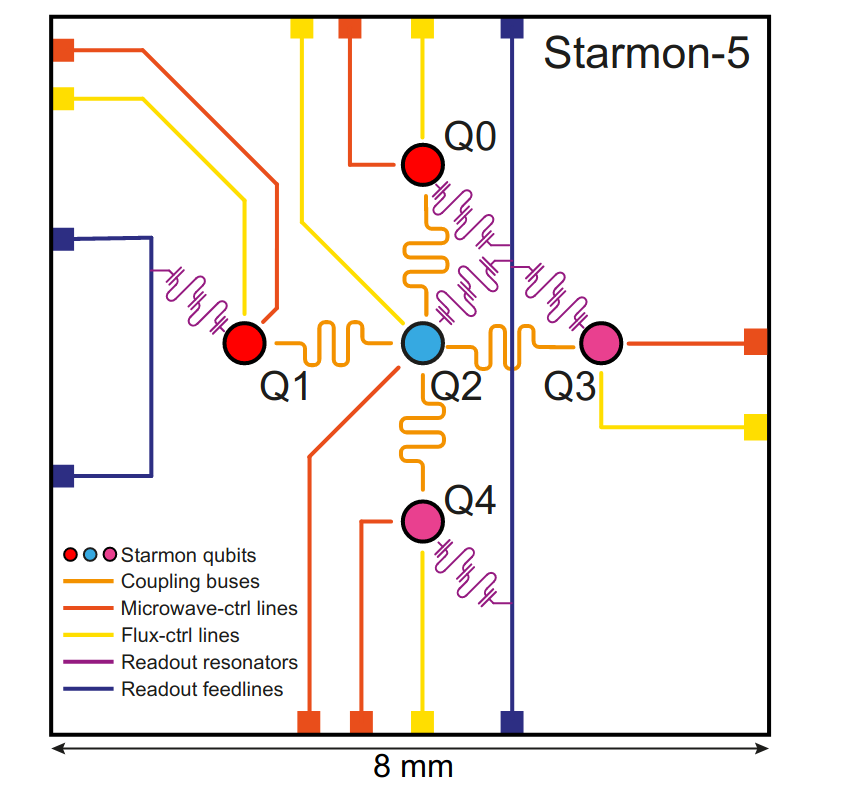
\includegraphics[width=.52\textwidth]{images/starmon5.png}   
  \captionsetup{width=.8\linewidth}
    \caption{Starmon 5 quantum processor. Retrieved from \cite{starmon_ref}}
    \label{starmon5}
    \end{minipage}

\end{figure}


\subsection{Layer by layer optmization}

Let's first consider the classical approach when running QAOA with $p$ layers. In this setting we have a circuit with $2p$ parameters, a $\gamma$ and a $\beta$ for each layer. Thus, the classical optimizer will optimize these $2p$ parameters all at once. This will be referred as \textit{standard optimization} from now on. Standar optimization works fine when $p$ is low, but the dimension of the solution parameter's space drastically increases for high $p$. This means the optimizer will likely need to compute many evaluations to the objective function. An illustration  can be seen in figure \ref{calls}, where the red line shows the number of calls made by the standard optimization for increasing $p$. 

\begin{figure}[h]
    \centering
    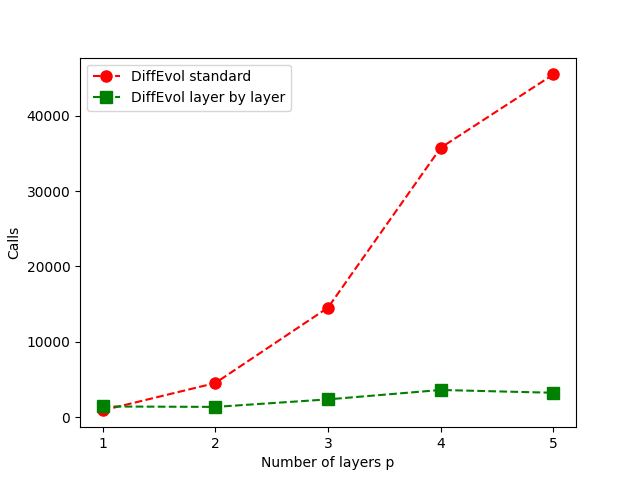
\includegraphics[width=0.5\linewidth]{images/Calls.png}    
    \caption{Number of calls to the objective function needed for standard and layer by layer optimization for increasing $p$}
    \label{calls}
\end{figure}

An alternative approach is the so called \textit{layer by layer} optimization. Let's again consider the case where we would like to run QAOA with $p$ layers. Withing this approach, we would first run the algorithm for $p=1$ and search for the optimum values of $\gamma_1, \beta_1$. Next, keeping the values for $\gamma_1, \beta_1$ fixed, we would run the algorithm for $p=2$ and optimize only the parameters for this layer $\gamma_2, \beta_2$. This process would be repeated $p$ times, optimizing the parameters of the ith-layer $\gamma_i \beta_i$ by keeping all the previous parameters  $\gamma_1, \beta_1 ... \gamma_{i-1}, \beta_{i-1}$ fixed. It is important to realize that now the dimension of the solution space is only 2 and not $2p$ like before, and that increasing $p$ does not imply that this dimension in increased, but rather that we will have to optimize $p$ times in a 2-dim solution space. Therefore, we would expect that the calls made to the objective function increases linearly with p. Indeed this can be seen in figure \ref{calls}.

% No we do not have any reference for layer by layer I think. It is something we came up with bro. That is the originality :P But on a serious note, I don't think there are references for that because it is not really QAOA anymore and this is a sacrifice we thought we would do.

\begin{figure}
    \centering
    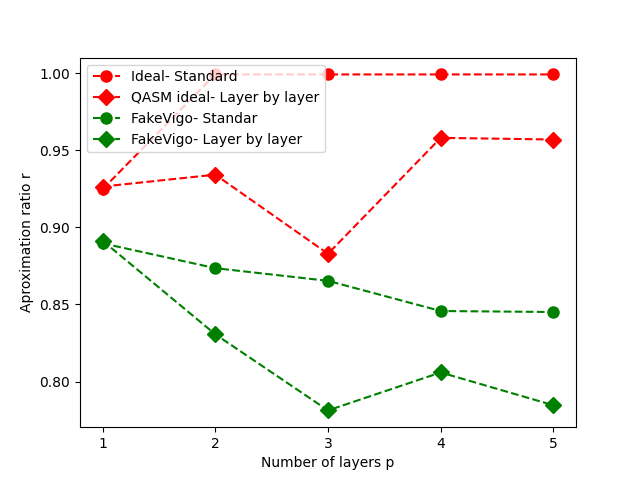
\includegraphics[width=0.6\linewidth]{images/layer by layer vs standard performance.png}
    \caption{Performance of the algorithm with standard and layer by layer optimization for increasing $p$. In red, for the QASM simulator with no noise and in green, for the FakeVigo simulator.}
    \label{performance layer standard}
\end{figure}

A final remark on the layer by layer optimization approach is that we are not considering the complete solution space but rather a subset of it. This means that the layer by layer optimization is not expected to reach a performance as high as the standard optimization. This is shown in figure \ref{performance layer standard}, where we compare the performance of the two optimization approaches in both the ideal QASM simulator and the FakeVigo simulator. Layer by layer optimization consistently achieves lower approximation ratios than the standard optimization for $p>1$ (for $p=1$ they are equivalent). 

One might be surprised to see, in figure \ref{performance layer standard}, that in the ideal case the performance drops for the ideal case in QASM for $p=3$. The performance in this ideal setting should be in principle at least as large as in the previous layer, since the optimizer should be able to choose $\gamma_3=0, \beta_3=0$, which would make the third layer to act as the identity, i.e. not perform any operations. The reason for this drop in $p=3$ is then probably due to the optimizer terminating the optimization before having found the optimal $\gamma_3, \beta_3$ as the maximum number of allowed iterations was reached.


\subsection{Choice of the optimizer}

There exists a wide variety of optimizers we can choose from. Current research is still vague on what optimizers will work best in this kind of hybrid quantum-classical algorithms like QAOA, so the choice of the optimizer usually takes an heuristic approach. Up until this section we used \textit{Differential-Evolution}, a global optimizer that has been shown to work well for QAOA \cite{alam2019analysis}. This is a global optimizer, which means it can avoid getting stuck in local minima, but on the other hand it usually takes many calls to the function. Other authors \cite{Lacroix_2020} have also used the local optimizers like \textit{Nelder-Mead} with satisfactory results. Additionally, Nelder-Mead needs to take less evaluation than Differential-Evolution. For this reason, Nelder-Mead was the chosen optimizer for running the algorithm in real backend


\subsection{Results}

We run QAOA for the Max-Cut on the 4-n 3-regular graph (figure \ref{fig:4ngraph}) in Vigo with up to 5 layers $(p=5)$. Even with the layer by layer optimization and using the Nelder-Mead optimizer, the whole code took around 2 days to run. Results can be seen in figure \ref{real_backend}. As expected, the overall performance for any $p$ in Vigo is lower than in FakeVigo, confirming that indeed this simulator heavily underestimates the errors in the real Vigo. On the other hand, FakeVigo did predict the qualitative behaviour of the algorith for $p>1$. Indeed we can see that, in the same way as in Vigo, the performance drops when adding more than one layer, unlike in the ideal case where the performance grows monotonically with $p$ (recall figure \ref{fig:statevector_graph}).
%I don't think we necessarily need a reference here. It can easily be seen that for greater p it should be at least as high as previous one. Maybe talk about that part earlier?


Additionally, we made use of QuTech's superconducting quantum processor, Starmon 5, consisting of 5 transmon qubits \cite{starmon_ref}. We were only able to run the algorithm for up to $p=3$ as the execution times in Starmon 5 when running deep circuits (recall that the depth of the circuit scales as $p$) were higher than in Vigo. The achieved performance in Starmon 5 was lower aswell. Error values aside, this fact is explained by the connectivity of the qubits in Starmon 5, which can be seen in figure \ref{starmon5}. It is easy to see that Vigo's topology is more adequate for the 4-n 3-regular graph, since less 2-qubit gates need to be applied between non connected qubits than in Starmon 5. This leads to more intermediate SWAP gates being applied, contributing to the overall error in the circuit. 


\begin{figure}
    \centering
    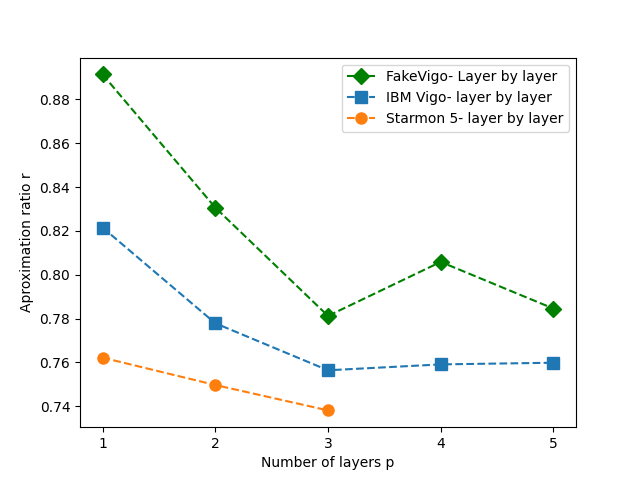
\includegraphics[width=0.6\linewidth]{images/starmon5 and vigo.png}    
    \caption{Performance of the algorithm in two real backends: Vigo from IBM Quantum Experience and Starmon 5 from QuTech, compared to that on the classical simulator FakeVigo.}
    \label{real_backend}
\end{figure}
%%%%%%%%%%%%%%%%%%%%%%%%%%%%%%%%%%%%%%%%%%%%%%%%%%%
The implementation of the project was done using the python library Qiskit. The code is available at \url{https://github.com/smitchaudhary/QAOA-MaxCut}.
